\section{Framework RL-Glue}
\label{RL-Glue}

\noindent
Aqu� se hablar� del framework (RL-Glue) y la biblioteca de ejemplos (RL-Library) que me ha permitido la implementaci�n del algoritmo Q-learning.

\subsection{RL-Glue}

\noindent
RL-Glue \cite{rl-glue} provee una interfaz est�ndar para que agentes, entornos y experimentos sean conectados en conjunto.

\vspace*{-0.5cm}
\begin{figure}[h!]
\centering
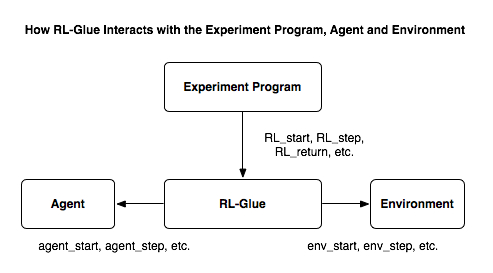
\includegraphics[scale=0.55]{imagen/glue_connections_no_shadow}
\caption{RL-Glue protocol}
\label{Fig:RL-Glue}
\end{figure}

% \noindent
Como se muestra en la figura \ref{Fig:RL-Glue}, los componentes necesarios son:
\begin{itemize}
 \item El \textbf{Agente}: programa que implementa el algoritmo de aprendizaje. En nuestro caso ser�a donde se ha implementado Q-Learning.
 \item El \textbf{Entorno}: programa que implementa la din�mica de la tarea, genera las observaciones y refuerzos. El entorno es, por ejemplo, un juego; en nuestro caso, el Tetris.
 \item El \textbf{Experimento}: programa encargado de la ejecuci�n de un experimento, incluida la secuencia de interacciones agente-entorno y la evaluaci�n del desempe�o del agente. El programa puede ser visual o en consola, para una evaluaci�n del rendimiento del agente m�s c�moda.
 \item El \textbf{RL-Glue Core}: programa que media la comunicaci�n entre el agente y el entorno en respuesta a los comandos guiados por el experimento.
\end{itemize}

% \noindent
El programa \textbf{Experimento} no debe tener acceso directo al \textbf{Agente} o el \textbf{Entorno}, todo contacto debe ir siempre primero a trav�s de la interfaz del \textbf{RL-Glue Core}. Tampoco hay contacto directo entre el agente y el entorno. Cualquier informaci�n que el agente o el entorno devuelva pasa a trav�s del RL-Glue al m�dulo que la necesite, seg�n se especifique en el protocolo.

RL-Glue ha sido usado tanto para ense�ar RL en varias universidades as� como tambi�n para crear experimentos cient�ficos publicados en conferencias l�deres.


\subsection{RL-Library}

La RL-Library \cite{RL-library} actualmente es una collecci�n de 10 entornos, 3 agents y 2 experimentos. Aqu� puede encontrarse el entorno usado (el Tetris) y el agente con una pol�tica \textit{random}, el cual fue un punto de partida interesante. El entorno usa una API, llamada RL-Viz, que es una capa arriba de RL-Glue que carga din�micamente el agente y el entorno, modificando par�metros en tiempo de ejecuci�n y visualizando la interacci�n y rendimiento.


